\documentclass[preprint,12pt,aps,pra,showkeys,amsmath,amssymb,superscriptaddress,floatfix]{revtex4-2}
\usepackage[T1]{fontenc}
\usepackage[utf8]{inputenc}
\usepackage{amsmath,amssymb,amsthm,mathtools,mathrsfs}
\usepackage{microtype,booktabs,enumitem}
\usepackage{xcolor,tikz,etoolbox}
\usepackage[skins,breakable]{tcolorbox}
\usepackage{needspace}
% Keep diagram geometry independent of REVTeX preprint body spacing.
\AtBeginEnvironment{tikzpicture}{\linespread{1}\selectfont}
\usetikzlibrary{arrows.meta,positioning,calc,fit,decorations.pathreplacing}
\usepackage{graphicx}
\usepackage{hyperref}

\definecolor{MMBlue}{RGB}{0,82,155}
\definecolor{MMOrange}{RGB}{200,80,0}
\tikzset{
 mmnode/.style={draw=MMBlue,rounded corners=2pt,fill=MMBlue!4,align=left,execute at begin node={\raggedright},text width=5cm,font=\fontsize{10}{12}\selectfont,inner sep=6pt},
 mmimport/.style={mmnode,draw=black!65,fill=black!4},
 mmcandidate/.style={mmnode,draw=MMOrange,dashed,fill=MMOrange!5},
 mmrejected/.style={mmnode,draw=black,densely dotted,fill=black!8},
 mmproof/.style={->,thick,MMBlue},
 mmflow/.style={->,semithick,black!70},
 mmrepair/.style={->,dashed,thick,MMOrange},
 mmcandidatearrow/.style={->,dashed,semithick,MMOrange},
 mmnote/.style={font=\scriptsize,fill=white,inner sep=2pt,align=center}}

\usepackage[section]{placeins}
\setlength{\emergencystretch}{3em}
\setlist{itemsep=3pt,topsep=4pt}
\newtheorem{theorem}{Theorem}[section]
\newtheorem{proposition}[theorem]{Proposition}
\newtheorem{lemma}[theorem]{Lemma}
\newtheorem{corollary}[theorem]{Corollary}
\theoremstyle{definition}
\newtheorem{definition}[theorem]{Definition}
\newtheorem{example}[theorem]{Example}
\theoremstyle{remark}
\newtheorem{remark}[theorem]{Remark}
% Avoid isolated statement headings and single-line paragraph fragments.
\BeforeBeginEnvironment{theorem}{\Needspace{6\baselineskip}}
\BeforeBeginEnvironment{definition}{\Needspace{5\baselineskip}}
\BeforeBeginEnvironment{proposition}{\Needspace{5\baselineskip}}
\BeforeBeginEnvironment{lemma}{\Needspace{5\baselineskip}}
\BeforeBeginEnvironment{corollary}{\Needspace{5\baselineskip}}
\clubpenalty=5000
\widowpenalty=5000
\newcommand{\R}{\mathbb R}\newcommand{\Z}{\mathbb Z}\newcommand{\N}{\mathbb N}
\newcommand{\Pa}{\operatorname{Pa}}\newcommand{\Desc}{\operatorname{Desc}}
\newcommand{\cl}{\operatorname{cl}}\newcommand{\cost}{\operatorname{cost}}
\newcommand{\status}{\operatorname{status}}
% Faculty cards: a visual rail groups the five faculties within one agent.
% The rail has no arrowhead and does not represent a proof dependency.
\newcommand{\mmfacultybadge}[1]{%
 \node[circle,draw=MMBlue,line width=1pt,fill=white,
 minimum size=7mm,inner sep=0pt,font=\sffamily\small\bfseries,text=MMBlue]
 at ([xshift=15pt,yshift=-15pt]frame.north west) {#1};}
\newcommand{\mmfacultyrail}{%
 \draw[MMBlue!80,line width=1pt]
 ([xshift=15pt,yshift=2pt]frame.north west)--
 ([xshift=15pt,yshift=-2pt]frame.south west);}
\newtcolorbox{mmfacultybox}[2]{enhanced,breakable,
 colback=MMBlue!4,colframe=MMBlue!4,boxrule=0pt,arc=3pt,
 left=39pt,right=9pt,top=4pt,bottom=4pt,
 before skip=2pt,after skip=2pt,
 fontupper=\small\linespread{1.1}\selectfont,
 overlay unbroken={\mmfacultyrail\mmfacultybadge{#1}},
 overlay first={\mmfacultyrail\mmfacultybadge{#1}},
 overlay middle={\mmfacultyrail},overlay last={\mmfacultyrail}}
\newcommand{\mmfaculty}[3]{%
 \begin{mmfacultybox}{#1}{#2}
 {\sffamily\bfseries\color{MMBlue}#2}\par\smallskip #3
 \end{mmfacultybox}}
\newcommand{\agent}[9]{%
 \Needspace{8\baselineskip}
 \subsubsection{#1}
 \noindent\textbf{Object.} #2\par
 \noindent\textbf{Role.} #3\par\smallskip
 \mmfaculty{E}{Ego}{#4}
 \mmfaculty{M}{Memory}{#5}
 \mmfaculty{I}{Intellect}{#6}
 \mmfaculty{S}{Sense}{#7}
 \mmfaculty{A}{Action}{#8}
 \smallskip\noindent #9\par}

\usepackage{longtable,array,calc}
\providecommand{\tightlist}{\setlength{\itemsep}{2pt}\setlength{\parskip}{0pt}}
\makeatletter
\def\frontmatter@abstract@produce{\par\addvspace{\frontmatter@preabstractspace}%
\begingroup\prep@absbox\unvbox\absbox\post@absbox\endgroup
\addvspace{\frontmatter@postabstractspace}}
\makeatother
\newcommand{\field}[2]{\par\smallskip\noindent\textbf{#1.} #2\par}
\setlength{\emergencystretch}{5em}
\AtBeginEnvironment{verbatim}{\small\linespread{1.0}\selectfont}


\hypersetup{colorlinks=true,linkcolor=MMBlue,urlcolor=MMBlue,pdfauthor={Dibakar Sigdel}}

\begin{document}

\title{Monotone Convergence Theorem\\[4pt]\large An End-to-End Meta-Math Walkthrough}

\author{Dibakar Sigdel}

\affiliation{Mindverse Computing LLC, Lynnwood, WA 98087, USA}

\date{October 2026}

\begin{abstract}

Test the limit against one simple function at a time. A factor \(c<1\)
makes the eventual comparison with \(f_n\) valid even where the limit
equals the test function. The report presents the target theorem,
declared imports, a dependency graph, five-faculty node contracts, a
continuous proof, a worked example, and a hypothesis-repair audit. It is
an authored mathematical exposition, not a deployed-agent transcript or
a formal proof-assistant certificate.

\end{abstract}\maketitle\linespread{1.12}\selectfont

\noindent\textbf{FA-01 / Functional Analysis and Measure Theory / Report v1}

\section{Target and import contract}

\begin{theorem}

On any measure space \((X,\Sigma,\mu)\), let \(f_n:X\to[0,\infty]\) be
measurable with \(f_n\le f_{n+1}\) everywhere. For \(f=\sup_n f_n\),
prove \(\int f\,d\mu=\lim_n\int f_n\,d\mu\), allowing \(+\infty\). No
finiteness or sigma-finiteness of \(\mu\) is assumed.

\end{theorem}

\subsection{Foundations and permitted imports}

Use countable additivity, continuity from below for measures, and the
definition
\(\int h=\sup\{\int s:0\le s\le h,\ s\text{ finite-valued measurable simple}\}\).
For disjoint measurable \(A_i\) and \(a_i\ge0\),
\(\int\sum_i a_i1_{A_i}=\sum_i a_i\mu(A_i)\), with \(0\cdot\infty=0\).
Continuity from below follows by decomposing an increasing union into
disjoint successive differences. Integral monotonicity follows directly
from the supremum definition.

\clearpage\section{Node interaction workflow}

\begin{center}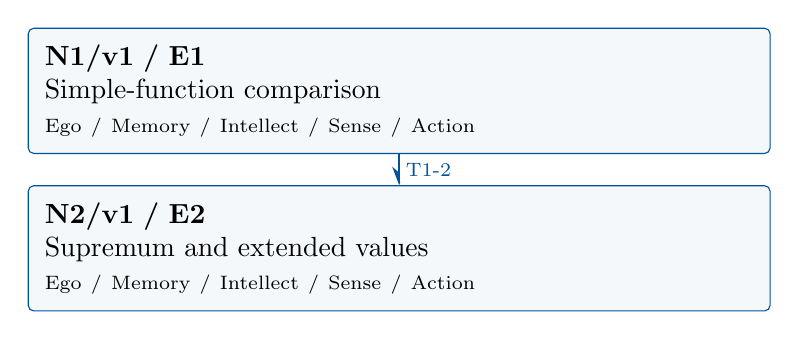
\begin{tikzpicture}[>=Stealth,x=1cm,y=1cm]

\node[mmnode,text width=9cm,minimum height=1.25cm] (N1) at (0,0.0) {\textbf{N1/v1 / E1}\\Simple-function comparison\\{\scriptsize Ego / Memory / Intellect / Sense / Action}};

\node[mmnode,text width=9cm,minimum height=1.25cm] (N2) at (0,-2.0) {\textbf{N2/v1 / E2}\\Supremum and extended values\\{\scriptsize Ego / Memory / Intellect / Sense / Action}};

\draw[mmproof] (N1.south) -- node[mmnote,right] {T1-2} (N2.north);

\end{tikzpicture}\end{center}

Each box is one mathematical agent containing all five faculties. Blue
arrows carry the versioned exports listed below. The layout gives a
reading order; only drawn arrows assert dependencies. Diagnostic repair
is separate from the proof DAG.

\subsection{Versioned evidence-transfer ledger}

\begingroup\small\linespread{1.05}\selectfont

\Needspace{5\baselineskip}\field{T1-2: N1/E1/v1 to N2}{For every such \(s\) and \(c\), \(\lim_n\int f_n\ge c\int s\).}

\field{Receiving activity}{N2.1}

\field{Compatibility}{E1/v1 and \(0\le f_n\le f\); the integral is defined by simple
minorants. Check: Never subtract two infinite integrals; handle the
extended-real comparison directly.}

\endgroup

\clearpage\section{Agent roles and five-faculty activities}\begingroup\small\linespread{1.05}\selectfont\setlist{itemsep=1pt,topsep=2pt}

\subsection{N1/v1: Simple-function comparison}

\field{Object and role}{Approximate the support of each positive level from below by places
where \(f_n\) has reached \(cs\). \textbf{Local obligation:} For every
such \(s\) and \(c\), \(\lim_n\int f_n\ge c\int s\).}

\field{Inputs}{A fixed simple \(s=\sum_{i=1}^m a_i1_{A_i}\le f\) with disjoint \(A_i\),
and \(0<c<1\).}

\mmfaculty{E}{Ego}{Publish E1/v1 only after establishing this obligation: For every such
\(s\) and \(c\), \(\lim_n\int f_n\ge c\int s\).}

\mmfaculty{M}{Memory}{A fixed simple \(s=\sum_{i=1}^m a_i1_{A_i}\le f\) with disjoint \(A_i\),
and \(0<c<1\). Retain the stated assumptions and import versions.}

\mmfaculty{I}{Intellect}{Approximate the support of each positive level from below by places
where \(f_n\) has reached \(cs\).}

\mmfaculty{S}{Sense}{At a point with \(s>0\), the strict margin \(cs<s\le f\) is essential;
do not claim eventual attainment of \(s\) itself.}

\mmfaculty{A}{Action}{Carry out activities N1.1--N1.2 below, retaining each calculation and
construction as evidence.}

\smallskip\noindent\textbf{Numbered mathematical activities}

\begin{enumerate}[label=N1.\arabic*,leftmargin=3.4em]

\item The supremum of measurable functions is measurable, so \(f\) is
measurable. Set \(B_n=\{x:f_n(x)\ge c s(x)\}\). These measurable sets
increase. Every point with \(s(x)>0\) lies in their union, since
otherwise \(f(x)\le cs(x)<s(x)\); points with \(s(x)=0\) already lie in
every \(B_n\).

\item Because \(cs1_{B_n}\le f_n\), monotonicity gives
\(\int f_n\ge c\sum_i a_i\mu(A_i\cap B_n)\). Continuity from below gives
\(\mu(A_i\cap B_n)\uparrow\mu(A_i)\). The sum has finitely many
nonnegative terms, so its limit is \(\int s\), also when a positive term
is infinite. This proves the export.

\end{enumerate}

\field{Export E1/v1}{For every such \(s\) and \(c\), \(\lim_n\int f_n\ge c\int s\).}

\field{Acceptance gate}{At a point with \(s>0\), the strict margin \(cs<s\le f\) is essential;
do not claim eventual attainment of \(s\) itself.}

\field{Targeted repair}{If a candidate uses \(c=1\), restore \(0<c<1\) and repeat the support
exhaustion before taking any limit. Withhold this export and recheck its
descendants after a versioned correction.}

\clearpage

\subsection{N2/v1: Supremum and extended values}

\field{Object and role}{Take the scalar limit \(c\uparrow1\), then the supremum over simple
functions. \textbf{Local obligation:} \(\lim_n\int f_n=\int f\) in
\([0,\infty]\).}

\field{Inputs}{E1/v1 and \(0\le f_n\le f\); the integral is defined by simple
minorants. Incoming proof exports: E1/v1 at N2.1.}

\mmfaculty{E}{Ego}{Publish E2/v1 only after establishing this obligation:
\(\lim_n\int f_n=\int f\) in \([0,\infty]\).}

\mmfaculty{M}{Memory}{E1/v1 and \(0\le f_n\le f\); the integral is defined by simple
minorants. Incoming proof exports: E1/v1 at N2.1. Retain the stated
assumptions and import versions.}

\mmfaculty{I}{Intellect}{Take the scalar limit \(c\uparrow1\), then the supremum over simple
functions.}

\mmfaculty{S}{Sense}{Never subtract two infinite integrals; handle the extended-real
comparison directly.}

\mmfaculty{A}{Action}{Carry out activities N2.1--N2.2 below, retaining each calculation and
construction as evidence.}

\smallskip\noindent\textbf{Numbered mathematical activities}

\begin{enumerate}[label=N2.\arabic*,leftmargin=3.4em]

\item Put \(L=\lim_n\int f_n\), which exists in \([0,\infty]\) because the
integrals increase. E1 gives \(L\ge c\int s\). If \(\int s<\infty\), let
\(c\uparrow1\) to obtain \(L\ge\int s\). If \(\int s=\infty\), any fixed
\(c>0\) already gives \(L=\infty\).

\item Taking the supremum over all simple \(s\le f\) yields \(L\ge\int f\).
Conversely \(f_n\le f\) gives \(\int f_n\le\int f\) for every \(n\), so
\(L\le\int f\). The two comparisons prove the asserted equality without
an infinity subtraction.

\end{enumerate}

\field{Export E2/v1}{\(\lim_n\int f_n=\int f\) in \([0,\infty]\).}

\field{Acceptance gate}{Never subtract two infinite integrals; handle the extended-real
comparison directly.}

\field{Targeted repair}{If infinity is treated as an ordinary real number, replace that
manipulation with the two order inequalities just proved. Withhold this
export and recheck its descendants after a versioned correction.}

\endgroup\clearpage\section{Continuous mathematical proof}\label{sec:proof}

\subsection{N1 --- Simple-function
comparison}\label{n1-simple-function-comparison}

\begin{enumerate}
\def\labelenumi{\arabic{enumi}.}
\item
  \textbf{N1.1.} The supremum of measurable functions is measurable, so
  \(f\) is measurable. Set \(B_n=\{x:f_n(x)\ge c s(x)\}\). These
  measurable sets increase. Every point with \(s(x)>0\) lies in their
  union, since otherwise \(f(x)\le cs(x)<s(x)\); points with \(s(x)=0\)
  already lie in every \(B_n\).
\item
  \textbf{N1.2.} Because \(cs1_{B_n}\le f_n\), monotonicity gives
  \(\int f_n\ge c\sum_i a_i\mu(A_i\cap B_n)\). Continuity from below
  gives \(\mu(A_i\cap B_n)\uparrow\mu(A_i)\). The sum has finitely many
  nonnegative terms, so its limit is \(\int s\), also when a positive
  term is infinite. This proves the export.
\end{enumerate}

\subsection{N2 --- Supremum and extended
values}\label{n2-supremum-and-extended-values}

\begin{enumerate}
\def\labelenumi{\arabic{enumi}.}
\item
  \textbf{N2.1.} Put \(L=\lim_n\int f_n\), which exists in
  \([0,\infty]\) because the integrals increase. E1 gives
  \(L\ge c\int s\). If \(\int s<\infty\), let \(c\uparrow1\) to obtain
  \(L\ge\int s\). If \(\int s=\infty\), any fixed \(c>0\) already gives
  \(L=\infty\).
\item
  \textbf{N2.2.} Taking the supremum over all simple \(s\le f\) yields
  \(L\ge\int f\). Conversely \(f_n\le f\) gives \(\int f_n\le\int f\)
  for every \(n\), so \(L\le\int f\). The two comparisons prove the
  asserted equality without an infinity subtraction.
\end{enumerate}

\hfill$\square$

\section{Worked orchestration}

For Lebesgue measure on \((0,1)\), take \(f_n(x)=\min(n,1/x)\). It
increases to \(1/x\). Splitting at \(1/n\) gives
\(\int_0^1 f_n=1+\log n\) for \(n\ge1\), hence the theorem correctly
returns \(\int_0^1 dx/x=\infty\). This exercises the extended-valued
conclusion.

\subsection{Boundary and hypothesis audit}

On \((0,1)\), \(g_n=n1_{(0,1/n)}\) tends pointwise to zero but has
integral one. The sequence is not increasing; pointwise convergence
alone cannot replace the monotonicity hypothesis.

\section{Illustrative failure and repair}

The following is an authored diagnostic scenario. Changed assumptions
define a new contract; they do not retroactively prove the original
statement.

\subsection{Rejected argument, diagnosis, and correction}
\textbf{Rejected candidate (N1.1):} \(s\le f\) implies eventually
\(s\le f_n\). Take \(s=f=1\) and \(f_n=1-1/(n+1)\). \textbf{Diagnosis:}
Intellect lost the strict comparison margin. \textbf{Repair:} compare
\(cs\) for \(c<1\), then use N2 to pass \(c\uparrow1\). This fills the
proof under the original hypotheses. Recheck E1 and E2; the target is
unchanged.

\subsection{Publication and reuse}
The corrected export retains its explicit assumptions. A hypothetical
revision receives a new version, and each consuming activity is
rechecked; this scenario is not a recorded runtime event. \textbf{Next
direction:} Use this export to prove Fatou's lemma by applying it to the
increasing tail infima of a nonnegative sequence.

\par\medskip\begingroup\small\linespread{1.0}\selectfont\noindent\textbf{Provenance.} This authored proof is complete relative to its declared imports. Reuse
each export with its assumptions, proof, and version. The original
Markdown remains available for comparison.
\par\endgroup

\par\smallskip\begingroup\small\linespread{1.0}\selectfont\noindent\textbf{Further reading.} \href{https://ocw.mit.edu/courses/18-102-introduction-to-functional-analysis-spring-2021/resources/lecture-notes/}{MIT
OpenCourseWare, Introduction to Functional Analysis: lecture notes}. See
the lectures on integration, Hilbert spaces, Baire category, and
Hahn--Banach.\par\endgroup

\end{document}
